% !TEX program = xelatex
% !TEX encoding = UTF-8
%============================================================================
% TrajVis Studio -- Project Proposal (Task 1)
% Course : Software Engineering -- 2026 Fall
% Group  : 1  /  Team: 泓泓说的都队
% Author : Chen Hongzhou (Student No. 1240007950), team leader
%============================================================================
\documentclass[12pt,a4paper]{report}

\usepackage{fontspec}
\setmainfont{Times New Roman}
\setsansfont{Helvetica}
\usepackage{xeCJK}
\setCJKmainfont{Songti SC}

\usepackage[a4paper,margin=2.5cm]{geometry}
\usepackage{graphicx}
\usepackage{booktabs}
\usepackage{array}
\usepackage{amsmath,amssymb}
\usepackage{xcolor}
\usepackage{float}
\usepackage{caption}
\usepackage{tikz}
\usetikzlibrary{positioning,arrows.meta,calc,fit,backgrounds}
\usepackage[hidelinks]{hyperref}

% Let long URLs break at slashes instead of running into the margin, and set
% them in the body font rather than the monospace one.
\urlstyle{same}
\makeatletter
\g@addto@macro\UrlBreaks{\do\/\do\-\do\.\do\_\do\:}
\makeatother

% Long identifiers and URLs should break instead of running into the margin.
\emergencystretch=3em

% --- Running header and footer -----------------------------------------
% Mirrors "Surface for project-2026.09.25.docx": every page carries the
% running title of its chapter at the left of the header over a dark rule
% (the template colours that rule 622423), and the page number centred in
% the footer.  The template has no header on the cover, which the
% titlepage environment already takes care of.
\usepackage{fancyhdr}
% Times New Roman at 12pt needs a taller header box than the 12pt default;
% take the extra height off \topmargin so the text block does not move down.
\setlength{\headheight}{25pt}
\addtolength{\topmargin}{-10pt}
\definecolor{mustrule}{HTML}{622423}
\newcommand{\surfacehead}{%
  \fancyhead[L]{\small\nouppercase{\leftmark}}%
  \fancyfoot[C]{\small\thepage}%
  \renewcommand{\headrulewidth}{1.1pt}%
  \renewcommand{\headrule}{%
    \hbox to\headwidth{\color{mustrule}%
      \leaders\hrule height \headrulewidth\hfill}}%
}
\pagestyle{fancy}
\fancyhf{}
\surfacehead
% Chapter-opening pages use the "plain" style; give it the same furniture.
\fancypagestyle{plain}{\fancyhf{}\surfacehead}
% Header text is "Chapter N <title>", unnumbered front matter just its title.
\def\chaptermark#1{\markboth{Chapter \thechapter\enspace #1}{}}
\def\sectionmark#1{\markright{\thesection\enspace #1}}

% Chapter-based numbering, e.g. "Figure 2-1", "Table 3-2"
\renewcommand{\thefigure}{\thechapter-\arabic{figure}}
\renewcommand{\thetable}{\thechapter-\arabic{table}}

% The template names these two sections "Table of Contents" and "References"
% rather than the class defaults "Contents" and "Bibliography".
\renewcommand{\contentsname}{Table of Contents}
\renewcommand{\bibname}{References}

% --- TikZ styles --------------------------------------------------------
\tikzset{
  pbox/.style={rectangle,draw,rounded corners,minimum height=0.78cm,
               align=center,font=\small,thick,inner sep=3pt},
  arr/.style={-{Stealth[length=2.5mm]},thick},
  back/.style={-{Stealth[length=2.5mm]},thick,dashed},
  part/.style={rectangle,draw,minimum height=0.62cm,align=center,
               font=\scriptsize,inner sep=2pt},
  grp/.style={rectangle,draw,dashed,rounded corners,inner sep=6pt}
}

\begin{document}

%============================================================================
% COVER PAGE  (layout follows "Surface for project-2026.09.25.docx")
%============================================================================
\begin{titlepage}
  \begin{tikzpicture}[remember picture, overlay]
    \foreach \off in {24, 26.5, 29} {
      \draw[line width=0.6pt]
        ([shift={(\off pt, -\off pt)}]current page.north west)
        rectangle
        ([shift={(-\off pt, \off pt)}]current page.south east);
    }
  \end{tikzpicture}

  \linespread{1.5}\selectfont
  \fontsize{15pt}{18pt}\selectfont
  \centering

  \vspace*{1.2cm}
  
\includegraphics[height=3cm]{logo.jpeg}

  \vspace{2\baselineskip}
  {\bfseries MACAU UNIVERSITY OF SCIENCE AND\\ TECHNOLOGY\par}

  \vspace{\baselineskip}
  {\bfseries School of Computer Science and Engineering\par}
  {\bfseries Faculty of Innovation Engineering\par}

  \vspace{2\baselineskip}
  % The template writes literal "<<" and ">>".  Two adjacent "<" are a T1
  % ligature that renders as the guillemet <<, so put an empty group between
  % them to stop the ligature from forming.
  {\bfseries <{}<{}Software Project for Course Software Engineering>{}>\par}

  \vspace{2\baselineskip}
  \parbox{\textwidth}{\hspace*{1.5cm}%
    \begin{tabular}{@{}l@{: }>{\raggedright\arraybackslash}p{10.5cm}@{}}
      Homework ID  & Task1-Project Proposal \\
      Report Title & TrajVis Studio: A Self-Service Platform for
                     Natural-Language Trajectory Analysis \\
      Group Number & 1 \\
      Team Members & \begin{tabular}[t]{@{}l@{\hspace{1.2em}}l@{}}
                       Chen Hongzhou & 1240007950 \quad (team leader) \\
                       Zhou Guoxi    & 1240007947 \\
                       Xu Jing       & 1240007919
                     \end{tabular} \\
      Date         & 2026.10.7 \\
    \end{tabular}}
\end{titlepage}

%============================================================================
% FRONT MATTER
%============================================================================
\chapter*{Abstract}
\addcontentsline{toc}{chapter}{Abstract}
\markboth{Abstract}{}

Cities, delivery companies and research groups now record the movement of
vehicles, riders and pedestrians in far greater detail than they can use.
The records contain the answers to questions that planners, transport
researchers and operations managers ask every week---which streets stayed busy
after nine in the evening, which districts a particular traveller visited, how
long a delivery round actually took. The people who ask those questions are
almost never the people who can query the data. Every question is handed to a
data specialist, answered by hand, drawn by hand, and returned as a picture.
The round trip takes days, and when somebody asks six months later how a figure
was produced, nobody can say.

This proposal diagnoses that round trip and proposes \textbf{TrajVis Studio}, a
system in which an analyst asks a question in ordinary language and receives a
figure together with the chain of reasoning that produced it. The system writes
the data request itself, retrieves the trajectories the question refers to,
chooses the chart that fits the question, summarises the result in a sentence,
and keeps a complete record that can be re-run later. A public benchmark of
9{,}608 recorded question-and-answer pairs is built into the system, so that its
accuracy is measured continuously instead of assumed.

The proposal is written in the order the course requires. Chapter~\ref{ch:diag}
diagnoses the problem, Chapter~\ref{ch:treat} prescribes the treatment, and
Chapter~\ref{ch:plan} sets out the plan of work, the team and the ownership of
each part of the product. The feasibility argument rests on work we have already
done rather than on optimism: a working prototype already runs on a single
laptop, reaching 64\% fully-correct answers against a 34\% baseline on a public
benchmark of 9{,}608 recorded questions, at no software or cloud cost. The
system is built to show that number rather than assert it---it re-runs the
benchmark on demand and reports its own measured accuracy beside every answer it
gives.

% The class already sets the running mark for these three lists, so no
% \markboth here: doing it beforehand would leak the next title onto the
% page being closed.
\tableofcontents
\addcontentsline{toc}{chapter}{Table of Contents}
\listoffigures
\addcontentsline{toc}{chapter}{List of Figures}
\listoftables
\addcontentsline{toc}{chapter}{List of Tables}

%============================================================================
\chapter*{Project Identification}
\addcontentsline{toc}{chapter}{Project Identification}
\markboth{Project Identification}{}

\begin{table}[H]
  \centering
  \begin{tabular}{@{}l@{\hspace{1.2em}}>{\raggedright\arraybackslash}p{11.0cm}@{}}
    \toprule[1.5pt]
    Project title   & TrajVis Studio: A Self-Service Platform for
                      Natural-Language Trajectory Analysis \\
    Group number    & 1 \\
    Topic category  & Self-chosen topic from a real-world problem
                      (Part A, option 1): a working tool for analysts who
                      cannot write queries themselves \\
    Team name       & 泓泓说的都队 (\emph{Honghong Is Always Right}) \\
    Team leader     & Chen Hongzhou \\
    Team members    & Chen Hongzhou, Zhou Guoxi, Xu Jing \\
    Repository      & \url{https://github.com/chenhongzhou666/MUST-SE-TrajVis} \\
    \bottomrule[1.5pt]
  \end{tabular}
\end{table}

%============================================================================
\chapter{Introduction}
\label{ch:intro}

\section{The setting}

Every bus, delivery van, patrol car and mobile phone leaves a trail of
timestamps and locations behind it. Ten years ago, storing those trails was the
difficult part; today they arrive by themselves, and the difficult part has
moved somewhere else. The trails are only worth keeping if somebody can ask
questions of them, and the people with the questions are not the people who can
operate the database.

A planner in a municipal transport bureau wants to know whether the evening
shuttle actually reaches the hospital district before the last clinic closes. A
researcher studying how a disease spreads wants the contact history of one
confirmed case. A logistics manager wants to know which of her riders is losing
forty minutes a day to the same junction. In each case the question is perfectly
clear when spoken aloud, and in each case answering it today means finding a
colleague who writes database queries for a living, waiting for a slot in that
colleague's queue, and accepting whatever picture comes back.

Those three situations are the real-world problem this project is built on. We
did not begin with a technique and look for somewhere to apply it; we began with
work that people do every week and cannot finish. Chapter~\ref{ch:diag} goes
back over each of them in more detail, and the measures in
Chapter~\ref{ch:treat} are stated in terms of them.

\section{Who this proposal is for}

The proposal is addressed to the person who pays for the analysis: the head of a
small planning, research or operations team. That customer does not want to hear
about query languages or chart libraries. The customer wants to know three
things---that we understand what is wrong today, that what we propose will
actually remove the problem, and that we can finish it. Chapters~\ref{ch:diag}
to~\ref{ch:plan} answer those three questions in that order.

\section{How to read this proposal}

Chapter~\ref{ch:diag} describes the problem domain and narrows it, step by step,
from the general situation above down to the five specific sub-problems this
project will address. Chapter~\ref{ch:treat} describes the system we propose to
build, the measures by which the customer will judge it, and its business value.
Chapter~\ref{ch:plan} gives the plan of work, the team, the ownership of each
part of the product, and a preliminary estimate of cost and completion date.

%============================================================================
\chapter{Problem Diagnosis}
\label{ch:diag}

\section{The problem domain: people who work with movement}

The three groups below are the users we have in mind. We chose them because they
share a single pattern: they hold the questions, they do not hold the data
skills, and their work is interrupted by the gap between the two.

\begin{table}[H]
  \centering
  \caption{The users we are proposing for, and the questions they ask.}
  \label{tab:users}
  \begin{tabular}{@{}p{3.6cm}p{5.2cm}p{6.2cm}@{}}
    \toprule[1.5pt]
    \textbf{User} & \textbf{Typical question} & \textbf{How the answer is used} \\
    \midrule
    Municipal transport planner & Was the evening shuttle still in the
      hospital district after the clinic closed last week? &
      To re-time a route before the next council meeting. \\
    \addlinespace
    Transport or epidemiology researcher & Which districts did this
      traveller pass through between March and May? &
      To establish a contact history and publish a finding. \\
    \addlinespace
    Fleet or delivery operations manager & Which rider lost the most
      time at the same junction this month? &
      To change a shift plan or a route assignment. \\
    \bottomrule[1.5pt]
  \end{tabular}
\end{table}

Common to all three is that the question arrives in words, but the answer lives
in a database. Everything that happens between those two points is what this
proposal is about.

\section{How the work is done today}

Figure~\ref{fig:today} shows the round trip as it happens in practice. It is worth
following one question through it, because the cost is not in any single step.

\begin{figure}[H]
  \centering
  \begin{tikzpicture}[node distance=0.62cm and 0.5cm]
    \node[pbox,text width=2.9cm] (a) {Analyst writes the question down in words};
    \node[pbox,text width=2.9cm,right=of a] (b) {Question waits in the
      specialist's queue};
    \node[pbox,text width=2.9cm,right=of b] (c) {Specialist writes a database
      query and runs it};
    \node[pbox,text width=2.9cm,below=of c] (d) {The answer comes back as a
      plain table of numbers};
    \node[pbox,text width=2.9cm,left=of d] (e) {Somebody decides which kind of
      chart to draw};
    \node[pbox,text width=2.9cm,left=of e] (f) {The chart is drawn by hand and
      sent back};
    \draw[arr] (a) -- (b);
    \draw[arr] (b) -- (c);
    \draw[arr] (c) -- (d);
    \draw[arr] (d) -- (e);
    \draw[arr] (e) -- (f);
    \draw[back] (f.west) -- ++(-0.75,0) |- (a.west);
    \node[font=\scriptsize,text width=9.0cm,align=center,anchor=north]
      at ([yshift=-2.8cm]$(a.south)!0.5!(c.south)$)
      {If the chart does not answer the question, the whole loop starts again.};
  \end{tikzpicture}
  \caption{The round trip as it is practised today.}
  \label{fig:today}
\end{figure}

Two features of that loop deserve attention. First, only two of the six steps
require the analyst's judgement; the rest is queueing and translation. Second,
the loop has no natural end---if the returned picture does not answer the
question, the whole cycle repeats, and the analyst discovers this only at the
end.

\section{What goes wrong}

We separate five issues. The first three are visible to the analyst; the last
two are visible to the organisation.

\subsection{The answer takes days, and almost all of that time is waiting}

A question that is fully formed in the analyst's head on Monday morning is
typically answered on Wednesday or later. Measured against the work actually
required---one query, one chart---the elapsed time is dominated by the queue in
front of the specialist. Because the delay is attached to the \emph{process}
rather than to any person, hiring more specialists moves the bottleneck without
removing it.

\subsection{The analyst cannot check the answer, only trust it}

The returned figure does not show what was actually asked. If the specialist
filtered on the wrong date column, or interpreted ``the hospital district'' as a
different district from the one the analyst meant, the figure will look
perfectly reasonable and will be wrong. The analyst has no way to notice. In our
domain a mis-scoped area or a misread time range is not a cosmetic error: it
changes the answer to the question.

\subsection{The chart is chosen by habit rather than by the question}

Which chart to draw is a consequence of what was asked. ``Which district did
this traveller visit'' asks for a map; ``how many vehicles were parked each
hour'' asks for a bar chart; ``how did the count change over the day'' asks for
a line. In current practice the choice is made by whoever draws the picture, and
a habitually-used chart type can hide the very pattern the analyst was looking
for. Nothing in the process ties the picture to the question.

\subsection{The work cannot be reproduced}

Six months later, when the same question is asked again or a figure is
challenged, the pieces needed to rebuild it are scattered: the original wording
lives in an e-mail, the query in somebody's editor history, the chart settings
nowhere at all, and the underlying data has since changed. Rebuilding the figure
means repeating the whole round trip and hoping the same answer comes out. For
research and for any decision that may later be audited, this is the most
expensive issue of the five, even though it is the least visible.

\subsection{Existing self-service tools stop one step short}

Reporting dashboards let an analyst pick a prepared chart, but they answer only
the questions somebody anticipated in advance, and they cannot express ``the
vehicles that were \emph{still} in the district after nine'', which is a
question about a sequence of positions rather than about a row in a table. Query
builders remove the queue but still require the analyst to know the schema and
the spatial vocabulary. Each tool moves the bottleneck rather than removing it,
because each one still requires the analyst to translate a spoken question into
the tool's own terms.

\section{The sub-problems this project will address}

The five issues above are too broad to be a project. We narrow them into the
five sub-problems below, and Chapter~\ref{ch:treat} proposes one treatment for
each.

\begin{table}[H]
  \centering
  \caption{From the issues observed today to the sub-problems we will work on.}
  \label{tab:issues}
  \begin{tabular}{@{}p{0.6cm}p{6.0cm}p{8.4cm}@{}}
    \toprule[1.5pt]
    & \textbf{Issue today} & \textbf{Sub-problem this project takes on} \\
    \midrule
    S1 & The spoken question must be translated by a person &
      Turn a question asked in ordinary language into an exact, written request
      that a machine can carry out and a person can read back. \\
    \addlinespace
    S2 & Answering requires knowing the schema and the spatial vocabulary &
      Find the trajectories the question refers to without the analyst knowing
      how the data is stored or how places are named inside it. \\
    \addlinespace
    S3 & The chart is chosen by whoever draws it &
      Choose the chart as a consequence of the question, and draw it without
      human intervention. \\
    \addlinespace
    S4 & Nothing can be rebuilt afterwards &
      Record every step of one exchange, so that the same figure can be produced
      again from the record alone. \\
    \addlinespace
    S5 & Whether the automation works is a matter of opinion &
      Measure the accuracy of the whole chain against recorded
      question-and-answer pairs, and show the measurement to the user. \\
    \bottomrule[1.5pt]
  \end{tabular}
\end{table}

%============================================================================
\chapter{Proposed Treatment}
\label{ch:treat}

\section{The system in one paragraph}

TrajVis Studio is a program the analyst runs on an ordinary machine. The analyst
types a question in plain language. The system replies with a figure, one
sentence saying what the figure shows, and a plain-language account of what it
understood the question to mean. If the question was ambiguous, the system asks
one clarifying question instead of guessing. Every exchange is stored, and a
stored exchange can be re-run to produce the same figure again. Alongside the
working system there is a measuring instrument: a set of 9{,}608 recorded
question-and-answer pairs on which the system's accuracy is computed and
displayed, so that the analyst can see how far the automation can be trusted
rather than being asked to take it on faith.

Figure~\ref{fig:system} shows the arrangement. The four steps in the middle are
what replaces the queue in Figure~\ref{fig:today}; the benchmark underneath is
what makes the result checkable rather than merely plausible.

\begin{figure}[H]
  \centering
  \begin{tikzpicture}[x=1cm,y=1cm]
    \node[pbox,text width=2.5cm] (q) at (0,0)
      {Question in ordinary language};
    \node[part,text width=2.7cm] (p1) at (4.3,1.35) {Interpret the question};
    \node[part,text width=2.7cm] (p2) at (4.3,0.45) {Find the trajectories};
    \node[part,text width=2.7cm] (p3) at (4.3,-0.45)
      {Choose the chart and draw it};
    \node[part,text width=2.7cm] (p4) at (4.3,-1.35) {Summarise the result};
    \node[grp,fit=(p1)(p4),
          label={[font=\small\bfseries]above:TrajVis Studio}] (sys) {};
    \node[pbox,text width=2.8cm] (out) at (8.9,0.65)
      {Figure, one sentence, and the request it used};
    \node[pbox,text width=2.8cm] (rec) at (8.9,-1.35)
      {Record that can be re-run later};
    \node[pbox,text width=3.1cm] (bm) at (4.3,-3.5)
      {Benchmark of 9{,}608 recorded pairs};
    \draw[arr] (q) -- (sys.west);
    \draw[arr] (sys.east) -- (out);
    \draw[arr] (out.south) -- (rec.north);
    \draw[arr] (bm.north) -- (sys.south)
      node[midway,left=0.15cm,font=\scriptsize,text width=2.6cm,align=right]
      {measures the accuracy of};
  \end{tikzpicture}
  \caption{The proposed system. Four steps replace the queue; the benchmark
    underneath is what turns ``it looks right'' into a number.}
  \label{fig:system}
\end{figure}

\section{What the analyst does, and what the system does}

The division of labour is the whole point of the proposal, so we state it
explicitly.

\begin{table}[H]
  \centering
  \caption{The split of work between the analyst and the system.}
  \label{tab:split}
  \begin{tabular}{@{}p{7.2cm}p{7.8cm}@{}}
    \toprule[1.5pt]
    \textbf{What the analyst does today} & \textbf{What the system does instead} \\
    \midrule
    Writes the question down for somebody else &
      Reads the question as it was spoken and writes the request itself \\
    \addlinespace
    Waits for the specialist, then re-explains if the answer is wrong &
      Answers immediately, and shows what it understood so the analyst can
      correct it on the spot \\
    \addlinespace
    Inspects a table of numbers and decides what it means &
      States in one sentence what the figure shows, including the largest and
      smallest values it found \\
    \addlinespace
    Decides which chart to draw, then draws it &
      Chooses the chart from the question and draws it \\
    \addlinespace
    Keeps no record, or keeps it in several places &
      Keeps one record per exchange, re-runnable later \\
    \bottomrule[1.5pt]
  \end{tabular}
\end{table}

The analyst's remaining job is the one that should have been theirs all along:
deciding whether the question was the right question.

\section{Three example scenarios}

\subsection{Re-timing an evening shuttle}

A planner asks: \emph{``Show me where the evening shuttle was between nine and
eleven at night, last Tuesday.''} The system answers with a map on which the
shuttle's positions in that window are drawn as a trail, and the sentence ``The
shuttle was still moving inside the hospital district until 22:40; it left the
district nine minutes later than the last scheduled clinic closing.'' The
planner did not name a chart, a district, or a time format. If the system is
unsure which Tuesday was meant, it asks before answering.

\subsection{Establishing a contact history}

A researcher asks: \emph{``Which districts did traveller 128 pass through
between March 2010 and May 2012?''} The system answers with a map of the
districts concerned and the order in which they were visited, and attaches the
written request it used, so the researcher can check that ``March 2010'' was
read as the first of March rather than the thirty-first.

\subsection{Asking a question the system cannot answer well}

An operations manager asks a question whose answer the system is not confident
about. Rather than returning a plausible-looking figure, the system says what it
understood, states its measured accuracy on questions of this kind, and offers
the two readings it considers most likely. The manager chooses. This behaviour
matters more than it may appear: it is the difference between a tool whose
mistakes are visible and one whose mistakes are silent.

\section{Functional features}

The following list is the product we propose to deliver. Each item is a feature
the user can exercise, not a component of the implementation.

\begin{itemize}
  \item \textbf{F1 --- Ask in ordinary language.} The user states a question in
    plain English or Chinese, and the system turns it into an exact written
    request covering the kind of chart, the area, the time window and the
    selection of objects.
  \item \textbf{F2 --- Automatic retrieval and filtering.} The system finds the
    trajectories the request refers to, resolves place names written in the
    question against the places as they are recorded in the data, and returns
    only the matching subset.
  \item \textbf{F3 --- Automatic chart selection and drawing.} The system
    chooses the chart type that fits the question and renders the figure without
    the user choosing a chart type or a plotting tool.
  \item \textbf{F4 --- Plain-language summary of the result.} The system
    describes what the figure shows in one or two sentences, including the
    extremes it found, so the user need not read numbers off the chart.
  \item \textbf{F5 --- Accuracy dashboard.} The system runs the recorded
    question-and-answer pairs on demand, computes its own accuracy, and shows
    the result beside the answers it gives in normal use.
  \item \textbf{F6 --- Record and re-run an exchange.} Every exchange is stored
    with the question, the request the system derived, the data snapshot
    identifier and the figure, and can be re-run later to reproduce the same
    figure in one step.
\end{itemize}

Two of those features are what make this more than a chart tool. F5 and F6 mean
the system carries its own experiment with it: it can re-run the recorded
benchmark at any time and say what it scored, and it can rebuild any past answer
from the record alone. The customer therefore does not have to take our accuracy
on trust, and does not have to take any individual figure on trust either. The
experiment is not a report we write at the end; it runs inside the product, on
demand, whenever somebody asks for it.

\section{How the customer will know it worked}

We commit to five measures. Each is stated so that the customer can check it
without our help, and each is measured on questions we did not choose.

\begin{table}[H]
  \centering
  \caption{The measures by which the customer can judge the delivered system.}
  \label{tab:metrics}
  \begin{tabular}{@{}p{0.9cm}p{4.4cm}p{4.3cm}p{5.0cm}@{}}
    \toprule[1.5pt]
    & \textbf{Measure} & \textbf{Today} & \textbf{What we commit to} \\
    \midrule
    M1 & Time from question to figure &
      Two to four days (the round trip in Figure~\ref{fig:today}) &
      Under five minutes for a single question, measured on twenty questions
      taken from the customer's own backlog. \\
    \addlinespace
    M2 & Share of questions answered without a person intervening &
      Zero, by construction &
      At least 80\% of the same twenty questions answered with no human
      intervention beyond reading the answer. \\
    \addlinespace
    M3 & Accuracy of the automatic interpretation &
      34\% of questions fully correctly interpreted (the simplest available
      method, measured by us) &
      64\%, the best result published for this task, which our working
      prototype already reaches on the same public benchmark. \\
    \addlinespace
    M4 & Reproducibility &
      Not possible in practice &
      Every figure in the record can be rebuilt from the record alone, with one
      command, to the same image. \\
    \addlinespace
    M5 & Analyst satisfaction &
      Not measured &
      At least 4 out of 5, on a short questionnaire completed by five or more
      analysts who did not take part in building the system. \\
    \bottomrule[1.5pt]
  \end{tabular}
\end{table}

Two remarks on these numbers. M3 is not a guess: 34\% and 64\% are results we
have already obtained on our own machine, and they are the reason we are
confident that the target is reachable. M2 is deliberately stricter than M3,
because a system that is right 64\% of the time is only useful if it says so on
the remaining 36\% rather than quietly inventing an answer.

\section{The business value}

For the customer, the value is not that a figure is produced more cheaply. It is
that the queue disappears and the analyst becomes self-sufficient.

\begin{itemize}
  \item \textbf{The waiting disappears.} Work that currently spans days is done
    in the course of the meeting in which the question arises.
  \item \textbf{The analysis team stops being a queue.} The specialists are
    freed from routine questions and spend their time on the questions that
    genuinely need them.
  \item \textbf{Answers become checkable.} Because the system shows what it
    understood, an error is caught when it is made rather than when it is
    published.
  \item \textbf{Answers become auditable.} A figure produced in March can be
    rebuilt in September from its own record.
  \item \textbf{The work stays on the customer's own machine.} Trajectory data
    is frequently personal and frequently sensitive. The system is designed to
    run locally, so adopting it does not mean shipping movement records to a
    third party.
\end{itemize}

\section{What we will reuse}

The course asks us to be explicit about the building blocks we intend to stand
on, because that is what makes an estimate believable. We list them with their
cost, and we distinguish what we have already made work from what we still have
to make work.

\begin{table}[H]
  \centering
  \caption{Existing building blocks, their cost, and our state of readiness.}
  \label{tab:reuse}
  \begin{tabular}{@{}p{4.4cm}p{1.5cm}p{4.8cm}p{3.9cm}@{}}
    \toprule[1.5pt]
    \textbf{Building block} & \textbf{Cost} & \textbf{What it gives us} &
    \textbf{Our state} \\
    \midrule
    A published benchmark of 9{,}608 recorded question-and-answer pairs
      & Free, public &
      A fixed set of questions to measure accuracy against, so that M3 can be
      checked by anybody &
      Already in use \\
    \addlinespace
    A published method that breaks the question into four smaller steps, and a
      published written form for the request
      & Free, public &
      Removes the guesswork from the hardest part of the system: we are
      implementing a known-good recipe rather than inventing one &
      Already reproduced, reaching 64\% \\
    \addlinespace
    Open-source models that read and write language, run on the local machine
      & Free &
      Interpreting the question and writing the summary, without sending data
      away and without a per-question fee &
      Three models already running locally \\
    \addlinespace
    An open-source model that measures how similar two questions are
      & Free &
      Finding previously answered questions that resemble the new one, which is
      how the accuracy is raised from 34\% to 64\% &
      Already in use \\
    \addlinespace
    Open-source map and chart rendering libraries
      & Free &
      Drawing the figure once the chart type has been chosen &
      To be integrated \\
    \addlinespace
    An ordinary laptop with 24\,GB of memory
      & Already owned &
      Running the whole system, including the language models, without a
      server &
      Available \\
    \bottomrule[1.5pt]
  \end{tabular}
\end{table}

We also state what we are \emph{not} going to do, since a proposal that
promises everything is a proposal that has not been thought through.

\begin{itemize}
  \item We will not build a general-purpose assistant for arbitrary data. The
    system is scoped to movement data with time and place.
  \item We will not attempt to match the accuracy of proprietary services on
    every kind of question. We measure ourselves in public on one benchmark and
    report what we find.
  \item We will not build a polished visual identity. The course asks for
    design, and the interfaces will be plain on purpose.
  \item We will not train a model from scratch. Our contribution is the
    arrangement of existing parts into a system an analyst can use.
\end{itemize}

\section{What we will write it in}

The system is written in Python. We name the language here on purpose. The
course asks that the project contain real programming rather than the assembly
of ready-made screens, and the language is where that requirement is met or
missed. Everything that carries the work is processing the machine does without
being told each step: reading the question and turning it into an exact request,
working out which trajectories that request refers to and returning only those,
deciding which chart fits the question and drawing it, scoring every answer
against the recorded benchmark, and keeping a record complete enough to re-run.
No part of the system is a screen that stores what a person types into a
database, and no part of it is a page that only displays text.

Python is not one of the four languages the course names as examples (C, C++,
Java, C\#), and we would rather say so than leave it to be discovered. Those
examples describe the usual case. The binding constraint is different here: we
build on a published method whose reference implementation is written in Python,
and staying in that language is the plain reason the accuracy figure in
Table~\ref{tab:metrics} is a number we can point to rather than a hope---we are
running the same recipe, not an approximation of it---and it removes a class of
uncertainty from the plan at no cost. If the customer would rather see the work
in one of the named languages, we can say now that this is a change we would
take on knowingly, at the price of that starting point.

%============================================================================
\chapter{Plan of Work and Product Ownership}
\label{ch:plan}

\section{The shape of the work}

The work divides into three kinds, and it is worth separating them because they
carry different risk.

The first kind is \emph{settling what to build}. This is Task 2 of the course,
and it is a real dependency rather than a formality: the twenty questions we
measure M1 and M2 on have to come from a real user, and the feature list above
will move once those users speak.

The second kind is \emph{building the six features}. Feature F1 and F2 sit on
the critical path: nothing can be demonstrated until a question can be turned
into a request and a request into a set of trajectories. F3, F4 and F6 depend on
them. F5 is deliberately independent---the benchmark harness measures the
interpretation step only, and it already runs.

The third kind is \emph{measuring and reporting}. This is not a phase at the
end; M1 to M5 are computed continuously from the first working version, because
the whole justification of the system is that its accuracy is visible.

\begin{figure}[H]
  \centering
  \begin{tikzpicture}[x=0.82cm,y=0.62cm]
    % month grid
    \foreach \x/\m in {0/Oct, 4.4/Nov, 8.8/Dec} {
      \draw[gray!45] (\x,0.75) -- (\x,-8.6);
      \node[font=\scriptsize\bfseries,anchor=south west] at (\x,0.75) {\m};
    }
    \draw[gray!60] (0,0.75) -- (13.2,0.75);
    % bars: row / start / length / label
    \foreach \y/\s/\l/\lab in {%
      0/0/3.2/Requirements,
      1/2.4/2.4/F1 Interpretation,
      2/3.2/2.6/F2 Retrieval,
      3/5.6/2.4/F3 Chart,
      4/6.0/2.4/F4 Summary,
      5/0.4/1.6/F5 Dashboard,
      6/7.6/3.2/F6 Record,
      7/0.4/12.6/Measurement,
      8/11.6/1.6/Hand-over%
    } {
      \fill[blue!18,draw=blue!55] (\s,-\y-0.26) rectangle (\s+\l,-\y+0.26);
      \node[font=\scriptsize,anchor=east] at (-0.18,-\y) {\lab};
    }
    % customer checkpoints
    \foreach \x/\n in {3.2/1, 8.8/2, 13.2/3} {
      \draw[red!70,thick,densely dashed] (\x,-0.1) -- (\x,-8.7);
      \node[font=\scriptsize,text=red!70,anchor=north] at (\x,-8.75) {(\n)};
    }
  \end{tikzpicture}
  \caption{Indicative schedule. The dashed lines are the points at which the
    customer is shown something: (1)~the twenty measurement questions and the
    M1--M2 baseline, (2)~the first end-to-end demonstration, (3)~hand-over.
    Bars fix the order and the dependencies rather than exact dates; the dates
    are confirmed against the course calendar in
    Section~\ref{sec:short-term}.}
  \label{fig:plan}
\end{figure}

\section{Short-term plan}
\label{sec:short-term}

The course asks for the next few weeks in detail. We give six weeks, because
beyond that the estimate would be invented.

\begin{table}[H]
  \centering
  \caption{The next six weeks.}
  \label{tab:shortterm}
  \begin{tabular}{@{}p{1.7cm}p{9.3cm}p{4.0cm}@{}}
    \toprule[1.5pt]
    \textbf{Week} & \textbf{What is produced} & \textbf{Owner} \\
    \midrule
    Week 1 & Task 2 requirements elicited from the assigned customer team and
      from two real analysts; the twenty measurement questions fixed &
      Whole team \\
    \addlinespace
    Week 2 & Feature list frozen against those requirements; the record format
      for F6 agreed, because every other feature writes into it &
      Whole team \\
    \addlinespace
    Week 3 & F1 working end to end on typed questions, with the derived request
      displayed to the user &
      Pair A \\
    \addlinespace
    Week 4 & F2 working: retrieval and filtering, with place names in the
      question resolved against the data &
      Pair A \\
    \addlinespace
    Week 5 & F3 working: the chart type chosen from the question and drawn
      without user input; F5 extended to cover the full chain &
      Pair A (F3), B (F5) \\
    \addlinespace
    Week 6 & First end-to-end demonstration on the twenty questions; M1, M2 and
      M3 measured for the first time and reported to the customer &
      Whole team \\
    \bottomrule[1.5pt]
  \end{tabular}
\end{table}

\section{Team profile}

We are three students. Every member takes part in every activity---requirements,
design, implementation, testing and documentation---and the work is divided by
feature rather than by role. Chen Hongzhou leads the team.

\begin{table}[H]
  \centering
  \caption{Team members.}
  \label{tab:team}
  \begin{tabular}{@{}p{4.2cm}p{3.4cm}l@{}}
    \toprule[1.5pt]
    \textbf{Name} & \textbf{Student No.} & \textbf{Role} \\
    \midrule
    Chen Hongzhou & 1240007950 & Team leader \\
    Zhou Guoxi & 1240007947 & Member \\
    Xu Jing & 1240007919 & Member \\
    \bottomrule[1.5pt]
  \end{tabular}
\end{table}

\subsection{Contributions to this proposal}

Chen Hongzhou wrote this proposal. The work after it will be divided among the
three members along the lines set out in Table~\ref{tab:ownership}.

\section{Product ownership}

Product ownership here means: for each feature in the list at the end of
Chapter~\ref{ch:treat}, there is one person the customer can go to. It does not
mean that only that person will write the code; work may be moved between us as
we learn what is difficult, and any such move will be reported.

The course describes ownership in pairs. With three members we form one pair and
one single owner, and we say so plainly rather than hiding it: Pair~A takes the
four features that lie on the critical path, and the third member takes the two
features that can be built, tested and measured independently of them. This is a
deliberate split. It means that if Pair~A is delayed, the measuring instrument
and the record are still progressing, and the customer still gets a
demonstration.

\begin{table}[H]
  \centering
  \caption{Ownership of the functional features and the qualitative property
    each sub-team commits to.}
  \label{tab:ownership}
  \begin{tabular}{@{}p{2.6cm}p{4.2cm}p{4.5cm}p{3.3cm}@{}}
    \toprule[1.5pt]
    \textbf{Sub-team} & \textbf{Features owned} & \textbf{Qualitative property}
      & \textbf{How it is checked} \\
    \midrule
    Pair~A \newline Chen Hongzhou \newline Zhou Guoxi &
      F1 Ask in ordinary language \newline F2 Retrieval and filtering \newline
      F3 Chart selection and drawing &
      A whole question is answered in under five minutes, and no movement
      record leaves the machine &
      Timed on the twenty measurement questions; the system is run with the
      network disconnected. \\
    \addlinespace
    Individual \newline Xu Jing &
      F4 Plain-language summary \newline F5 Accuracy dashboard \newline
      F6 Record and re-run an exchange &
      An analyst who did not build the system can understand a result and
      rebuild it unaided &
      Five or more analysts complete the questionnaire and rebuild one figure
      from its record without help. \\
    \bottomrule[1.5pt]
  \end{tabular}
\end{table}

\section{Why three people}

The problem is worth three people and not fewer for a reason we can state
concretely. The work contains two halves that fail independently: the answering
chain (F1 to F3) and the measuring instrument (F4 to F6). The measuring
instrument is what makes the answering chain trustworthy, and it is the half
that is always dropped when a team is short of people. With three members we can
staff both halves at once. Two members would mean choosing between shipping a
demonstration and shipping evidence that the demonstration works, which is
exactly the trade-off this proposal exists to refuse.

Three is also enough and not too many, given the size: the work is roughly one
person per feature group over a semester, and the parts are separable along the
lines given above, so nobody is blocked waiting for somebody else for long.

\section{Preliminary estimate of cost and completion}

\begin{table}[H]
  \centering
  \caption{Preliminary cost estimate.}
  \label{tab:cost}
  \begin{tabular}{@{}p{5.4cm}p{9.4cm}@{}}
    \toprule[1.5pt]
    \textbf{Item} & \textbf{Estimate} \\
    \midrule
    Software licences & None. Every building block in
      Table~\ref{tab:reuse} is free and open source. \\
    \addlinespace
    Cloud or per-question fees & None. The language models run on the
      customer's own machine, which is also what keeps the movement data
      private. \\
    \addlinespace
    Data acquisition & None. The benchmark is public. Any additional movement
      data comes from the customer. \\
    \addlinespace
    Hardware & Already available: one laptop-class machine with 24\,GB of
      memory. No server is required. \\
    \addlinespace
    Effort & Approximately 180 person-hours: three members, about six hours
      per week each, over ten weeks. \\
    \addlinespace
    Completion & The system is demonstrated end to end in Week~6; the measured
      version, with M1 to M5 reported, is handed over at the end of the
      semester. \\
    \bottomrule[1.5pt]
  \end{tabular}
\end{table}

The estimate is preliminary and will be revised once the customer's
requirements are in hand; we expect the revision to affect the feature list more
than the cost, because the fixed costs are zero and the variable cost is our own
time.

\section{How we will report progress}

The course requires source code on GitHub and progress reports on Feishu, and we
treat both as commitments to the customer rather than as coursework
bookkeeping.

\begin{itemize}
  \item \textbf{Source code} is kept at
    \url{https://github.com/chenhongzhou666/MUST-SE-TrajVis}, with one
    directory per feature so that the boundaries in the ownership table are
    visible in the repository itself.
  \item \textbf{A progress report is posted on Feishu every week}, stating what
    moved, what did not, and what the current measurement of M1 to M3 is. The
    measurement is included every week, including in the weeks when it has not
    improved.
  \item \textbf{Every member reports their own part.} The course asks that each
    member demonstrate the whole process of their tasks, so each weekly report
    names what each of the three contributed, not only what the team achieved.
\end{itemize}

\section{Risks}

\begin{table}[H]
  \centering
  \caption{The three risks we consider material, and our response.}
  \label{tab:risks}
  \begin{tabular}{@{}p{5.2cm}p{9.6cm}@{}}
    \toprule[1.5pt]
    \textbf{Risk} & \textbf{Response} \\
    \midrule
    The requirements turn out to demand features outside the six listed. &
      The feature list is frozen in Week~2, before implementation starts, and
      changes after that are traded against features already owned rather than
      added to the end. \\
    \addlinespace
    Accuracy on the customer's own questions is lower than on the benchmark. &
      Already anticipated: the benchmark questions and the customer's questions
      are different populations. M3 is reported on both, separately, so the gap
      is visible instead of being averaged away. \\
    \addlinespace
    A member becomes unavailable. &
      The ownership split is deliberately unbalanced towards Pair~A, and the
      measuring instrument is independent of the answering chain. Losing one
      member degrades the demonstration but leaves the evidence intact. \\
    \bottomrule[1.5pt]
  \end{tabular}
\end{table}

%============================================================================
\chapter{Conclusion}
\label{ch:concl}

The problem is not that trajectory data is hard to store. It is that the
questions people have about it are trapped behind a translation step that only a
few people can perform, and each translation costs days. TrajVis Studio removes
that step: the analyst asks in ordinary language, the system writes the request,
finds the trajectories, chooses the chart, draws it, says what it shows, and
keeps a record that can be re-run.

We have been careful in this proposal to claim only what we can support. The
accuracy target is not an aspiration but a number our prototype already reaches
on our own machine, and the system is built to keep proving it rather than to
state it once. The building blocks are all free. The one genuinely uncertain
part of the work---whether the customer's twenty questions resemble the
benchmark questions---has been made visible as a measurement rather than hidden
as an assumption, and will be reported weekly.

What we ask the customer to accept is therefore narrow and specific: a system
that answers in minutes what takes days today, that shows its own accuracy
instead of asserting it, and that leaves behind a record of every answer it
gave.

%============================================================================
% REFERENCES
%============================================================================
% \begin{thebibliography} opens with \chapter*, i.e. it starts a fresh page,
% so the ToC entry has to be written on that new page or it would record the
% page number of the last page of the Conclusion.
\begin{thebibliography}{9}
\phantomsection
\addcontentsline{toc}{chapter}{References}

\bibitem{bai2026}
H. Bai, J. Wei, et al. ``Text-to-TrajVis: Enabling Trajectory Data
Visualizations from Natural Language Questions.'' In \emph{Findings of the
Association for Computational Linguistics: ACL 2026}, pp.~19456--19475, 2026.

\bibitem{trajvl}
Text2Vis. \emph{dataset-TrajVL}: the public benchmark used in this proposal.
\url{https://github.com/Text2Vis/dataset-TrajVL}, 2026.

\bibitem{pressman}
R. S. Pressman. \emph{Software Engineering: A Practitioner's Approach}.
McGraw-Hill, 2009.

\bibitem{bruegge}
B. Bruegge and A. H. Dutoit. \emph{Object-Oriented Software Engineering Using
UML, Patterns, and Java}. 3rd edition, Pearson, 2013.

\end{thebibliography}

\end{document}
